\documentclass[aspectratio=169]{beamer}

\usepackage[texlive=2020]{atlasphysics}
\usepackage{booktabs, array}
\usepackage{siunitx}
\usepackage{/home/lacey/Documents/ATLAS/ANA-EXOT-2019-31-INT1/ANA-EXOT-2019-31-INT1-defs}

\def\Put(#1,#2)#3{\leavevmode\makebox(0,0){\put(#1,#2){#3}}}
\unitlength=1cm

\usefonttheme{serif}
\beamertemplatenavigationsymbolsempty
\setbeamertemplate{itemize items}[circle]

\setbeamertemplate{footline}[text line]{
	\leavevmode
	\begin{beamercolorbox}[wd=\paperwidth, ht=4ex, left]{author in head/foot}
	\usebeamerfont{author in head/foot}
	\setlength{\tabcolsep}{0pt}
	\begin{tabular}{
		>{\raggedright\arraybackslash} p{0.3\paperwidth}
		>{\centering\arraybackslash} p{0.4\paperwidth}
		>{\raggedleft\arraybackslash} p{0.3\paperwidth}}
		\phantom{---} \today & Lacey Rainbolt, University of Chicago & {\insertframenumber} / {\inserttotalframenumber} \phantom{---} \\
	\end{tabular}
	\smallskip
	\end{beamercolorbox}
}

\DeclareSIUnit{\Gbps}{Gbps}


\begin{document}


\begin{frame}{Feb.~3 loopback tests}

	\begin{itemize}
		\item Performed internal and external loopback tests \\[.5cm]
		\item Clock rate: \SI{156.25}{\mega\hertz} (reference clock used for transceivers) \\[.5cm]
		\item Test pattern: PRBS7 \\[.5cm]
		\item Data rate: \SI{10}{\Gbps} \\[.5cm]
		\item Main 16 transceivers implemented in project (3 are functioning) \\[.5cm]
		\item Project uses TFM framework
	\end{itemize}

\end{frame}


\begin{frame}{Internal loopback tests}
\centering

	\begin{tabular}{c c c}
		\textbf{Link 0} & \textbf{Link 7} & \textbf{Link 15} \\[.25cm]
		$56 / 89$ & $56 / 111$ & $55 / 93$ \\[.25cm]
		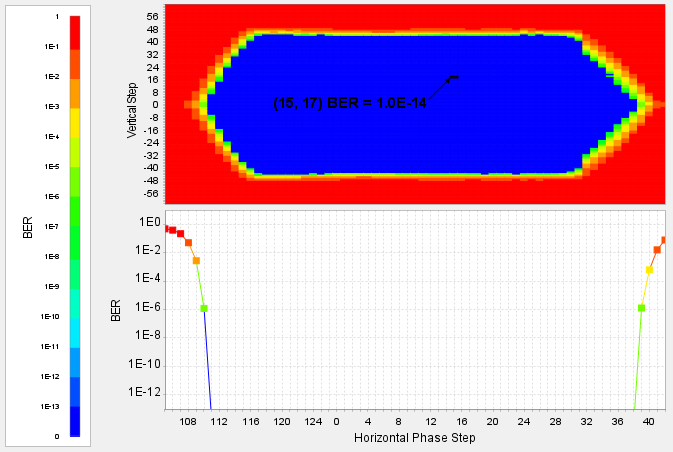
\includegraphics[width=.3\textwidth]{fig/2021-02-15_10g_prbs7_link0_lb.png} &
		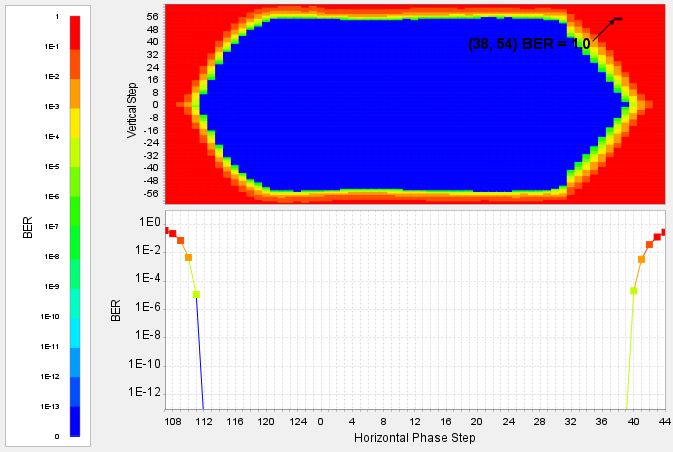
\includegraphics[width=.3\textwidth]{fig/2021-02-15_10g_prbs7_link7_lb.png} &
		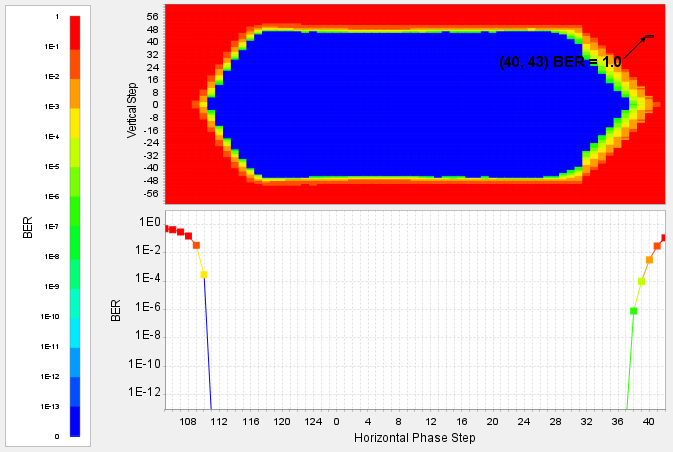
\includegraphics[width=.3\textwidth]{fig/2021-02-15_10g_prbs7_link15_lb.png}
	\end{tabular}
	
	\vspace{0.5cm}
	
	Currently we are not sure which link corresponds to which SMAs (Kade will check)

\end{frame}


\begin{frame}{External loopback tests}
\centering

	\begin{tabular}{c c c}
	\textbf{Link 0} & \textbf{Link 7} & \textbf{Link 15} \\[.25cm]
		$34 / 31$ & no eye & $22 / 43$ \\[.25cm]
		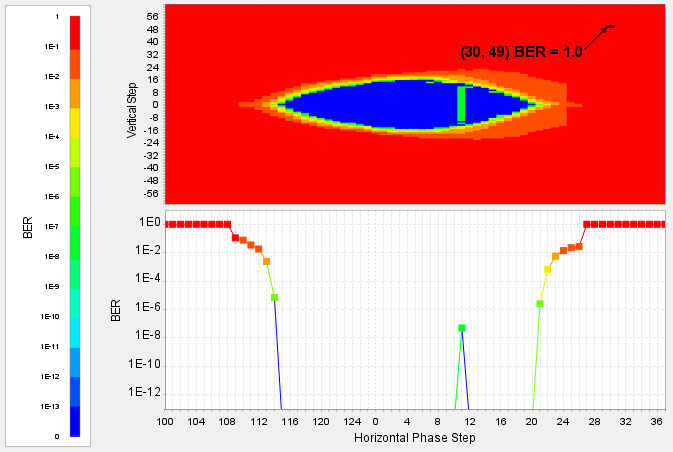
\includegraphics[width=.3\textwidth]{fig/2021-02-15_10g_prbs7_link0.png} &
		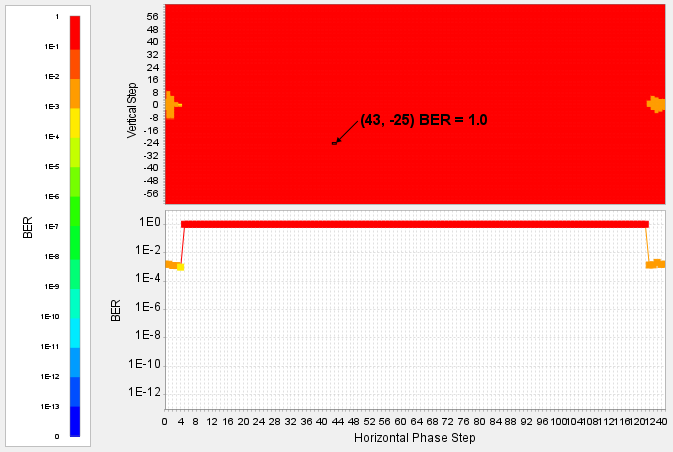
\includegraphics[width=.3\textwidth]{fig/2021-02-15_10g_prbs7_link7.png} &
		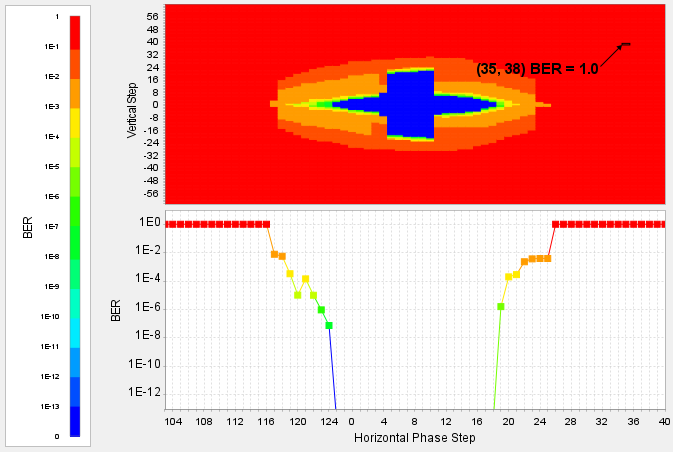
\includegraphics[width=.3\textwidth]{fig/2021-02-15_10g_prbs7_link15.png}
	\end{tabular}
	
	\vspace{0.5cm}
	
	These diagrams looked very strange, so we tried power cycling

\end{frame}


\begin{frame}{External loopback tests (after power cycling)}
\centering

	\vspace{.375cm}

	\begin{tabular}{c c c}
	\textbf{Link 0} & \textbf{Link 7} & \textbf{Link 15} \\[.25cm]
		$33 / 29$ & $22 / 11$ & $41 / 44$ \\[.25cm]
		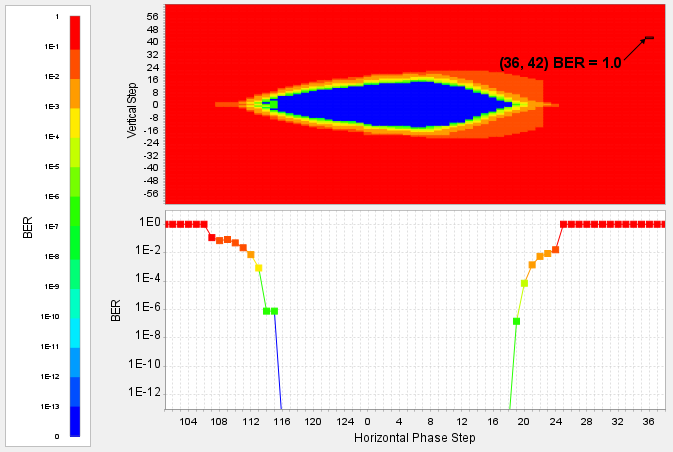
\includegraphics[width=.3\textwidth]{fig/2021-02-15_10g_prbs7_link0_powercycle.png} &
		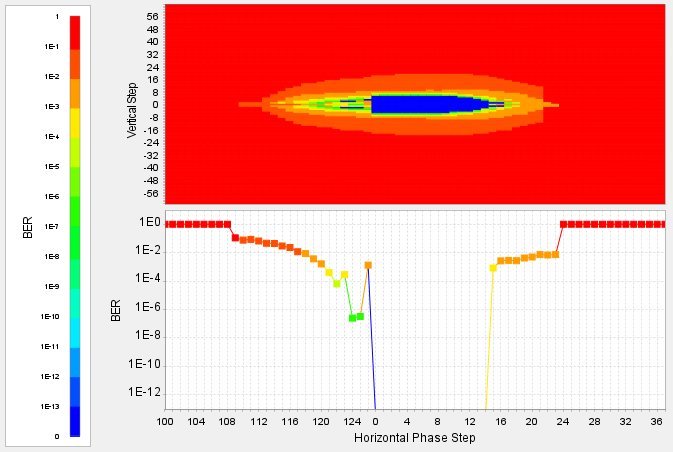
\includegraphics[width=.3\textwidth]{fig/2021-02-15_10g_prbs7_link7_powercycle.png} &
		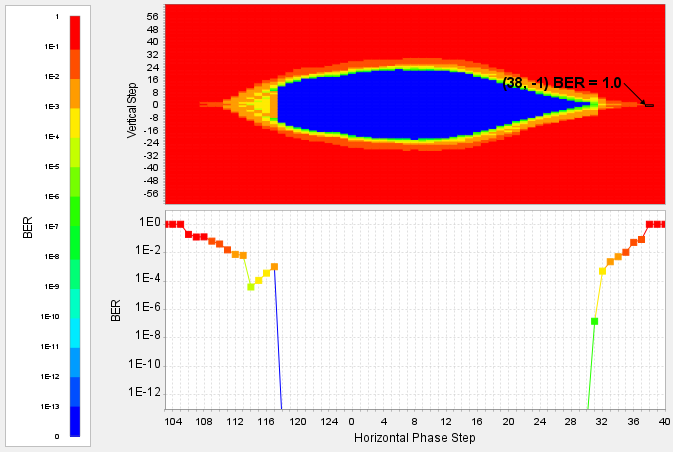
\includegraphics[width=.3\textwidth]{fig/2021-02-15_10g_prbs7_link15_powercycle.png}
	\end{tabular}
		
	\vspace{.25cm}
	
	\begin{itemize}
		\item Look better, but still not great (especially link 7)
		\item This Friday we will try a project with 64-bit interfacing
	\end{itemize}

\end{frame}


\end{document}